%% This file is generated by Jinja2
% Template for bipartite weighted matching
% Author: Long Gong
\documentclass[border=2pt]{standalone}
%%%<
\usepackage{verbatim}
%%%>
\begin{comment}
:Title: Template for bipartite weighted matching
:Author: Long Gong

A template for bipartite weighted matching. 

In some ways, this TeX script works as the "model" of our application 
for visualizing a weighted bipartite matching. 


Programmed in TikZ by Long Gong. Templating language is Jinja2, 
templaing syntax is the default setting of Jinja2.
\end{comment}


\usepackage{tikz}
\usetikzlibrary{calc,positioning}

\begin{document}
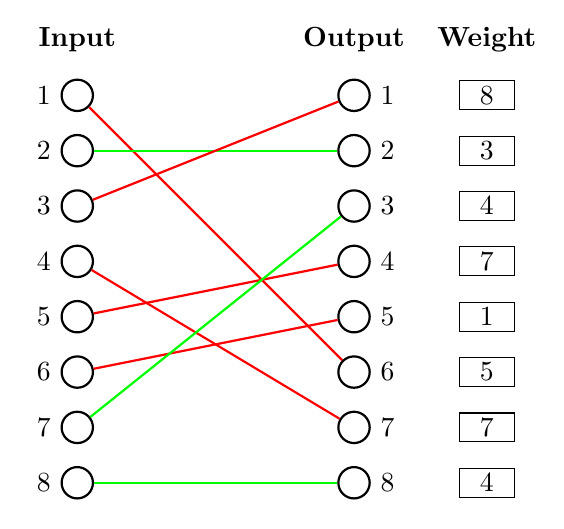
\begin{tikzpicture}[
vertex/.style={circle, draw, inner sep=4pt, thick},
edge/.style={thick},
weight/.style={rectangle, draw, inner sep=2pt, minimum width=20pt},
info/.style={draw=none,fill=none,inner sep=0pt}]

%% local variables
\def \margin{48pt}
\def \hm {100pt}
\def \vm {20pt}
\def \NUMOFVERTICES {8} 

%% place all input vertices
\foreach \s in {1,...,\NUMOFVERTICES}
      \node[vertex,label=left:$\s$] (I-\s) at (0,{- (\s - 1) * \vm}) {};

%% place all output vertices
\foreach \s in {1,...,\NUMOFVERTICES}
      \node[vertex,label=right:$\s$] (O-\s) at (\hm,{- (\s - 1) * \vm}) {};

\node[info] (I) at (0,{- (\NUMOFVERTICES - 1) * \vm}) {};
\node[info] (O) at (\hm,{- (\NUMOFVERTICES - 1) * \vm}) {};

%% place other ifnormation
\node[info] (in) at (0,\vm) {\bf Input};
\node[info] (out) at (\hm, \vm){\bf Output};
\node[info] (weight) at ({\hm+\margin}, \vm) {\bf Weight};

%% matching information
% ==========================================
% 1 6 5
% 2 2 3
% 3 1 8
% 4 7 7
% 5 4 7
% 6 5 1
% 7 3 4
% 8 8 4
% ==========================================

%% place all weight right of output vertices
%% previous version failed to change to place the weight near o instead of i
\node[weight] (W-6) at ({\hm+\margin},{- (5) * \vm}) {$5$};
%% previous version failed to change to place the weight near o instead of i
\node[weight] (W-2) at ({\hm+\margin},{- (1) * \vm}) {$3$};
%% previous version failed to change to place the weight near o instead of i
\node[weight] (W-1) at ({\hm+\margin},{- (0) * \vm}) {$8$};
%% previous version failed to change to place the weight near o instead of i
\node[weight] (W-7) at ({\hm+\margin},{- (6) * \vm}) {$7$};
%% previous version failed to change to place the weight near o instead of i
\node[weight] (W-4) at ({\hm+\margin},{- (3) * \vm}) {$7$};
%% previous version failed to change to place the weight near o instead of i
\node[weight] (W-5) at ({\hm+\margin},{- (4) * \vm}) {$1$};
%% previous version failed to change to place the weight near o instead of i
\node[weight] (W-3) at ({\hm+\margin},{- (2) * \vm}) {$4$};
%% previous version failed to change to place the weight near o instead of i
\node[weight] (W-8) at ({\hm+\margin},{- (7) * \vm}) {$4$};

%% place all edges
\foreach \i/\o/\c in {1/6/red, 2/2/green, 3/1/red, 4/7/red, 5/4/red, 6/5/red, 7/3/green, 8/8/green}
      \draw[edge,\c] (I-\i) -- (O-\o);

\end{tikzpicture}
\end{document}